\documentclass[russian]{lecture-notes}

\usepackage{misccorr}
\usepackage{graphicx}
\usepackage{amsmath}
\usepackage{systeme}
\usepackage{hyperref}
\usepackage{timestamps}
\usepackage{graphicx}
\graphicspath{{pic/}}
\usepackage{tikz}
\usepackage{algorithm}
\usepackage{algpseudocode}

\title{Транзитивное замыкание.
Алгоритм Уоршалла. Теорема Эйлера. Планарные графы.}

% указываем автора лекций. Несколько человек разделяются командой \and
\lecturer{Сергей Николаевич Поздняков}

\notesauthor{В.В.Пронин}

% начало документа
\begin{document}
\youtubevideo{S\_3xEmNwkFw}

\maketitle
\newpage

\section{Транзитивное замыкание}

\timestamp{1:30}

\begin{example}
    Допустим, у нас есть бинарное отношение (на рисунке пример отношения, заданного графом)
    \begin{figure}[H]
        %pic 1
        \centering
        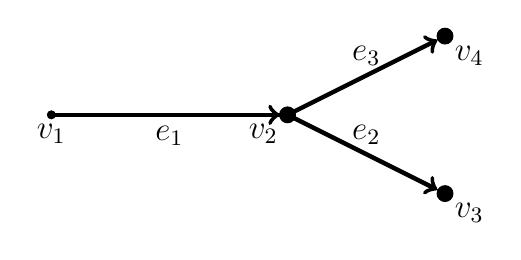
\begin{tikzpicture}[font = \large]
            \draw[ultra thick, ->] (0,0) -- (2.9,0);
            \draw[ultra thick, ->] (3,0) -- (4.9,0.95);
            \draw[ultra thick, ->] (3,0) -- (4.9,-0.95);
            
            \draw[ultra thick, ->]
            (0,0) -- node[below]{$e_1$}
            (3,0) -- node[]{} cycle;
            
            \draw 
            (3,0) -- node[above]{$e_3$}
            (5,1) -- node[]{} cycle;
            
            \draw 
            (3,0) -- node[above]{$e_2$}
            (5,-1) -- node[]{} cycle;
            
            \draw [fill = black] (0,0) circle(0.5mm) node[below]{$v_1$};
            \draw [fill = black] (3,0) circle(1mm) node[below left]{$v_2$};
            \draw [fill = black] (5,1) circle(1mm) node[below right]{$v_4$};
            \draw [fill = black] (5,-1) circle(1mm) node[below right]{$v_3$};
        \end{tikzpicture}
    \end{figure}
\end{example}

Является ли данное отношение транзитивным ? 

Вы скажете, что не является, потому что из $v_1$ можно попасть в $v_2$ по ребру $e_1$, а из $v_2$ в $v_3$ по ребру $e_2$, значит по транзитивности должно быть ребро из $v_1$ в $v_3$, а его нет. Добавим ребро.

\begin{figure}[H]
    %pic 2
    \centering
    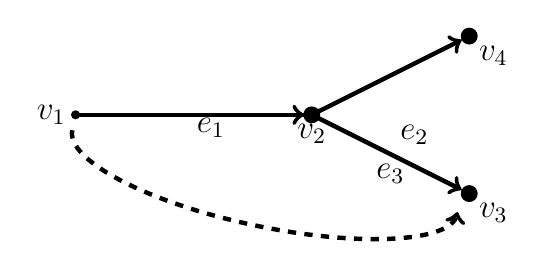
\begin{tikzpicture}[font = \large]
        \draw[ultra thick, ->] (0,0) -- (2.9,0);
        \draw[ultra thick, ->] (3,0) -- (4.9,0.95);
        \draw[ultra thick, ->] (3,0) -- (4.9,-0.95);
        
        \draw [ultra thick, ->, dashed, rotate = -12] (0,-0.2) arc (180:0:2.5 and -0.7);
        
        \draw[ultra thick, ->]
        (0,0) -- node[below right = -3pt]{$e_1$}
        (3,0) -- node[]{} cycle;
        
        \draw 
        (3,0) -- node[below = 1cm]{$e_3$}
        (5,1) -- node[]{} cycle;
        
        \draw 
        (3,0) -- node[above right]{$e_2$}
        (5,-1) -- node[]{} cycle;
        
        \draw [fill = black] (0,0) circle(0.5mm) node[left]{$v_1$};
        \draw [fill = black] (3,0) circle(1mm) node[below]{$v_2$};
        \draw [fill = black] (5,1) circle(1mm) node[below right]{$v_4$};
        \draw [fill = black] (5,-1) circle(1mm) node[below right]{$v_3$};
    \end{tikzpicture}
\end{figure}

А чего еще не хватает?

(Студенты предлагают добавить новые ребра).

\begin{figure}[H]
        %pic 1
        \centering
        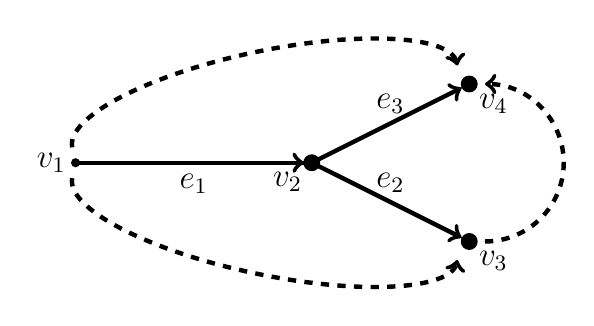
\begin{tikzpicture}[font = \large]
            \draw[ultra thick, ->] (0,0) -- (2.9,0);
            \draw[ultra thick, ->] (3,0) -- (4.9,0.95);
            \draw[ultra thick, ->] (3,0) -- (4.9,-0.95);
            
            \draw [ultra thick, ->, dashed] (5.2,-1) arc (90:-90:1 and -1);
            
            \draw [ultra thick, ->, dashed, rotate = 12] (0,0.2) arc (180:0:2.5 and 0.7);
        
            \draw [ultra thick, ->, dashed, rotate = -12] (0,-0.2) arc (180:0:2.5 and -0.7);
        
            \draw[ultra thick, ->]
            (0,0) -- node[below]{$e_1$}
            (3,0) -- node[]{} cycle;
            
            \draw 
            (3,0) -- node[above]{$e_3$}
            (5,1) -- node[]{} cycle;
            
            \draw 
            (3,0) -- node[above]{$e_2$}
            (5,-1) -- node[]{} cycle;
            
            \draw [fill = black] (0,0) circle(0.5mm) node[left]{$v_1$};
            \draw [fill = black] (3,0) circle(1mm) node[below left]{$v_2$};
            \draw [fill = black] (5,1) circle(1mm) node[below right]{$v_4$};
            \draw [fill = black] (5,-1) circle(1mm) node[below right]{$v_3$};
        \end{tikzpicture}
\end{figure}

Ребро из $v_3$ в $v_4$ можно было не добавлять и без него нет противоречий с транзитивностью.

\begin{figure}[H]
    %pic 2
    \centering
    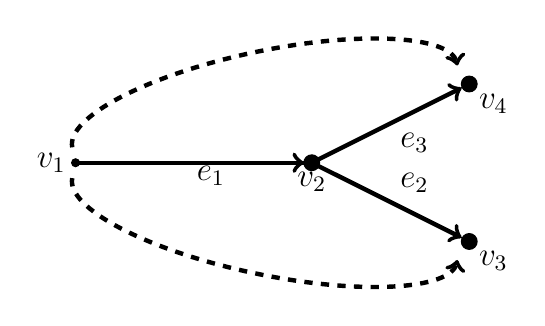
\begin{tikzpicture}[font = \large]
        \draw[ultra thick, ->] (0,0) -- (2.9,0);
        \draw[ultra thick, ->] (3,0) -- (4.9,0.95);
        \draw[ultra thick, ->] (3,0) -- (4.9,-0.95);
        
        \draw [ultra thick, ->, dashed, rotate = 12] (0,0.2) arc (180:0:2.5 and 0.7);
        
        \draw [ultra thick, ->, dashed, rotate = -12] (0,-0.2) arc (180:0:2.5 and -0.7);
        
        \draw[ultra thick, ->]
        (0,0) -- node[below right = -3pt]{$e_1$}
        (3,0) -- node[]{} cycle;
        
        \draw 
        (3,0) -- node[below right]{$e_3$}
        (5,1) -- node[]{} cycle;
        
        \draw 
        (3,0) -- node[above right]{$e_2$}
        (5,-1) -- node[]{} cycle;
        
        \draw [fill = black] (0,0) circle(0.5mm) node[left]{$v_1$};
        \draw [fill = black] (3,0) circle(1mm) node[below]{$v_2$};
        \draw [fill = black] (5,1) circle(1mm) node[below right]{$v_4$};
        \draw [fill = black] (5,-1) circle(1mm) node[below right]{$v_3$};
    \end{tikzpicture}
\end{figure}


\timestamp{3:30}
Поэтому транзитивным замыканием будет называться не любое согласованное с исходным транзитивное отношение, а только то, которое является общей частью всех согласованных транзитивных отношений, то есть будет минимальным из всех.

\timestamp{4:51}

\begin{definition}
    $T$ - называется транзитивным замыканием отношения $R$, если:
    \begin{enumerate}
    \item $T$ - транзитивно.
    \item $T$ - согласовано с $R$ (все отношения, которые были, остаются, а к ним добавляются новые).
    \begin{note}
        Для представления отношения графом это означает, что мы только добавляем ребра, ничего не убирая. Для представления матрицей это означает, что мы только добавляем единицы, опять же не убирая их.
    \end{note}
    \item Если $T'$ другое транзитивное и согласованное с $R$ отношение, то $T \in T'$.
    \end{enumerate} 
\end{definition}

\timestamp{6:40}

Для создания алгоритма транзитивного замыкания попробуем оттолкнуться от задания матрицы отношения и посмотрим нельзя ли использовать операцию умножения матриц для транзитивного замыкания.

Допустим, что у нас есть матрица, которую мы умножаем на себя. Напомню, что при этом $i$-тая строка скалярно умножается на $j$-тый столбец и на пересечении $i$-той строки и  $j$-того столбца записывается результат.
\begin{equation*}
\left(
\begin{array}{ccccc}
& & \vdots & &\\
& & \vdots & &\\
& & \vdots & &\\
& & \vdots & &\\
& & \vdots & &\\
\end{array}
\right)
\cdot
\left(
\begin{array}{ccccc}
& & & & \\
& & & & \\
\ldots & \ldots & \ldots & \ldots & \ldots\\
& & & & \\
& & & & \\
\end{array}
\right)
=
\left(
\begin{array}{ccccc}
& & \vdots & &\\
& & \vdots & &\\
\ldots& \ldots & \fbox{} & \ldots & \ldots\\
& & \vdots & &\\
& & \vdots & &
\end{array}
\right)
\end{equation*}

\timestamp{8:00}
В формальной записи в $i$-ой строке и $j$-ом столбце будет стоять элемент:
 
\[r_{i1} \cdot r_{1j} + r_{i2} \cdot r_{2j} + \ldots +r_{in} \cdot r_{nj}\]

Рассмотрим произведение $r_{i1} \cdot r_{1j}$. Индексы $i,1,j$ обозначают номера элементов множества или номера вершин графа. В терминах графа это произведение можно рассматривать как проверку того, можно ли пройти из $i$ в $j$ через вершину $1$. Если $r_{i1}$ равно $1$ и $r_{1j}$ равно $1$ (есть ребра из $i$ в $1$ и из $1$ в $j$, то их произведение будет равно $1$ (есть путь из $i$ в $j$ через $1$. Тогда сумма - элемент с индексами $i, j$ будет ненулевым, если из $i$ в $j$ можно попастпь через какую-либо из всех вершин.
 
Однако тогда результирующая матрица не обязательно будет являться матрицей смежностей (матрицей отношения), так как в ней могут присутствовать числа больше $1$. Нетрудно понять, что числа в этой матрице показывают сколькими способами мы можем пройти из одной вершины в другую через какие-то промежуточные вершины, а таких способов может быть больше одного. Поэтому мы будем использовать операцию $max$ вместо сложения.

\[r_{i1} \cdot r_{1j} + r_{i2} \cdot r_{2j} + \ldots +r_{in} \cdot r_{nj} \rightarrow max\{r_{i1} \cdot r_{1j};\ldots;r_{in} \cdot r_{nj}\}\]

Может возникнуть еще одна проблема, которую мы рассмотрим на примере.

\timestamp{10:30}
Допустим, у нас есть следующий граф
\begin{figure}[H]
    %pic 3
    \centering
    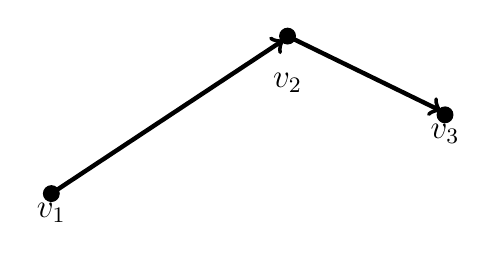
\begin{tikzpicture}[font = \large]
        \draw[ultra thick, ->] (0,0) -- (2.95,1.95);
        \draw[ultra thick, ->] (3,2) -- (4.95,1.05);
        
        \draw [fill = black] (0,0) circle(1mm) node[below]{$v_1$};
        \draw [fill = black] (3,2) circle(1mm) node[below = 10 pt]{$v_2$};
        \draw [fill = black] (5,1) circle(1mm) node[below]{$v_3$};
    \end{tikzpicture}

матрица отношений для этого графа:
    $\begin{pmatrix}
      0 & 1 & 0\\
      0 & 0 & 1\\
      0 & 0 & 0
    \end{pmatrix}
    $.    
\end{figure}

\begin{itemize}
\item Первая строка матрицы показывает, что из вершины $v_1$ можно попасть в вершину $v_2$, однако нельзя попасть в вершину $v_3$.
\item Вторая строка, аналогично первой, показывает, что из вершины $v_2$ можно попасть только в вершину $v_3$.
\item А третья строка показывает, что из вершины $v_3$ никуда нельзя попасть.
\end{itemize}

\timestamp{10:50}

При перемножении данной матрицы на себя получится матрица, которая показывает возможность из одной вершины попасть в какую-либо другую не напрямую, а через другие вершины графа.

$$\begin{pmatrix}
  0 & 1 & 0\\
  0 & 0 & 1\\
  0 & 0 & 0
\end{pmatrix}
\cdot
\begin{pmatrix}
  0 & 1 & 0\\
  0 & 0 & 1\\
  0 & 0 & 0
\end{pmatrix}
=
\begin{pmatrix}
  0 & 0 & 1\\
  0 & 0 & 0\\
  0 & 0 & 0
\end{pmatrix}
$$

\begin{figure}[H]
    %pic 4
    \centering
    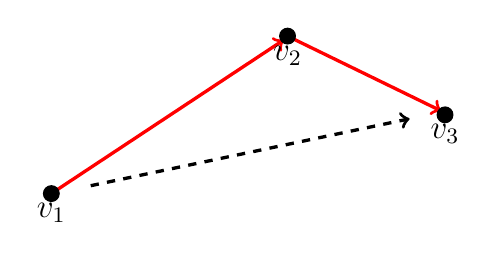
\begin{tikzpicture}[font = \large]
        \draw[very thick, ->,red] (0,0) -- (2.95,1.95);
        \draw[very thick, ->,red] (3,2) -- (4.95,1.05);
        \draw[very thick, ->, dashed] (0.5,0.1) -- (4.55,0.95);
        
        \draw [fill = black] (0,0) circle(1mm) node[below]{$v_1$};
        \draw [fill = black] (3,2) circle(1mm) node[below]{$v_2$};
        \draw [fill = black] (5,1) circle(1mm) node[below]{$v_3$};
    \end{tikzpicture}
\end{figure}

\timestamp{12:10}
Однократное умножение по новым правилам показывает достижимость одних вершин из других ровно за 2 шага.  Однако при этом мы теряем возможность узнать, возможно ли попасть в какую-либо вершину напрямую (показано красным).

\timestamp{12:25}
Для того, чтобы исправить данную ситуацию, необходимо добавить каждой вершине петлю (ребра, ведущие из вершин в себя, на рисунке обозначены синим цветом). Теперь из вершины $v_1$ в вершину $v_2$ можно добраться не напрямую, а  пройдя сначала по петле из вершины $v_1$ в саму себя, а потом в вершину $v_2$, таким же образом за 2 шага можно добраться из вершины $v_2$ в вершину $v_3$.

\begin{figure}[H]
    %pic 5
    \centering
    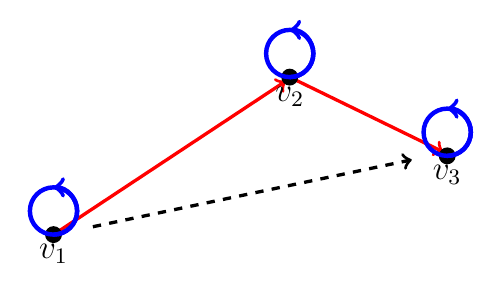
\begin{tikzpicture}[font = \large]
        \draw[very thick, ->,red] (0,0) -- (2.95,1.95);
        \draw[very thick, ->,red] (3,2) -- (4.95,1.05);
        \draw[very thick, ->, dashed] (0.5,0.1) -- (4.55,0.95);
        
        \draw [fill = black] (0,0) circle(1mm) node[below]{$v_1$};
        \draw [fill = black] (3,2) circle(1mm) node[below]{$v_2$};
        \draw [fill = black] (5,1) circle(1mm) node[below]{$v_3$};
        
        \draw[ultra thick, blue,rotate = -90] (0,0) arc (360:0:0.3);
        \draw[ultra thick, ->, blue,rotate = -90] (0,0) arc (0:180:0.3);
        \draw[ultra thick, blue,rotate = -90] (-2,3) arc (360:0:0.3);
        \draw[ultra thick, ->, blue,rotate = -90] (-2,3) arc (0:180:0.3);
        \draw[ultra thick, blue,rotate = -90] (-1,5) arc (360:0:0.3);
        \draw[ultra thick, ->, blue,rotate = -90] (-1,5) arc (0:180:0.3);
    \end{tikzpicture}
\end{figure}

Наше вычисление после добавления петель изменится следующим образом
$$\begin{pmatrix}
  1 & 1 & 0\\
  0 & 1 & 1\\
  0 & 0 & 1
\end{pmatrix}
\cdot
\begin{pmatrix}
  1 & 1 & 0\\
  0 & 1 & 1\\
  0 & 0 & 1
\end{pmatrix}
=
\begin{pmatrix}
  1 & (1) & 1\\
  0 & 1 & (1)\\
  0 & 0 & 0
\end{pmatrix}
$$
\begin{note}
    (1) означает, что в данную вершину можно попасть несколькими способами благодаря петлям, которые позволяют делать "холостые" перемещения из вершины в себя.
\end{note}

\timestamp{15:00}

 Для замыкания более сложного графа одного умножения будет недостаточно. Если по этому же правилу делать умножение матрицы следующего графа:

\begin{figure}[H]
    \centering
    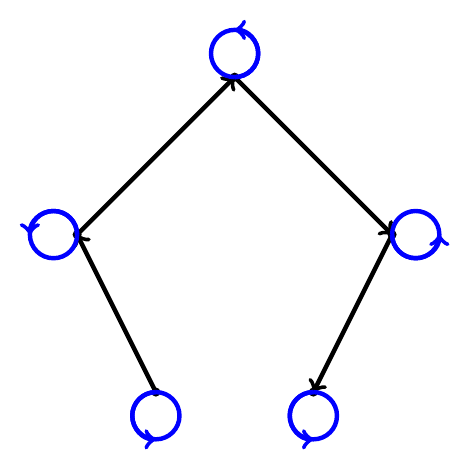
\begin{tikzpicture}[font = \large]
        \draw[ultra thick, ->] (0,0) -- (-1,2);
        \draw[ultra thick, ->] (-1,2) -- (1,4);
        \draw[ultra thick, ->] (1,4) -- (3,2);
        \draw[ultra thick, ->] (3,2) -- (2,0);
        
        \draw [fill = black] (0,0) circle(0.5mm);
        \draw [fill = black] (2,0) circle(0.5mm);
        \draw [fill = black] (3,2) circle(0.5mm);
        \draw [fill = black] (1,4) circle(0.5mm);
        \draw [fill = black] (-1,2) circle(0.5mm);
        
        \draw[ultra thick, blue,rotate = -270] (0,0) arc (360:0:0.3);
        \draw[ultra thick, ->, blue,rotate = -270] (0,0) arc (0:180:0.3);
        
        \draw[ultra thick, blue,rotate = -0] (-1,2) arc (360:0:0.3);
        \draw[ultra thick, ->, blue,rotate = -0] (-1,2) arc (0:180:0.3);
        
        \draw[ultra thick, blue,rotate = -90] (-4,1) arc (360:0:0.3);
        \draw[ultra thick, ->, blue,rotate = -90] (-4,1) arc (0:180:0.3);
        
        \draw[ultra thick, blue,rotate = -180] (-3,-2) arc (360:0:0.3);
        \draw[ultra thick, ->, blue,rotate = -180] (-3,-2) arc (0:180:0.3);
        
        \draw[ultra thick, blue,rotate = -270] (0,-2) arc (360:0:0.3);
        \draw[ultra thick, ->, blue,rotate = -270] (0,-2) arc (0:180:0.3);
        \end{tikzpicture}
\end{figure}

то после первого умножения добавятся ребра к вершинам, до которых можно добраться через одну промежуточную, при этом имеющиеся ребра сохранятся за счет того, что отношение стало рефлексивным

\begin{figure}[H]
    \centering
    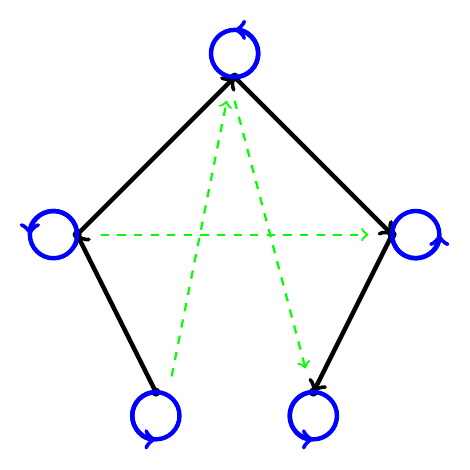
\begin{tikzpicture}[font = \large]
        \draw[ultra thick, ->] (0,0) -- (-1,2);
        \draw[ultra thick, ->] (-1,2) -- (1,4);
        \draw[ultra thick, ->] (1,4) -- (3,2);
        \draw[ultra thick, ->] (3,2) -- (2,0);
        
        \draw[thick, ->, dashed, green] (0.2,0.2) -- (0.9,3.7);
        \draw[thick, ->, dashed, green] (-0.7,2) -- (2.7,2);
        \draw[thick, ->, dashed, green] (1,3.7) -- (1.9,0.3);
        
        \draw [fill = black] (0,0) circle(0.5mm);
        \draw [fill = black] (2,0) circle(0.5mm);
        \draw [fill = black] (3,2) circle(0.5mm);
        \draw [fill = black] (1,4) circle(0.5mm);
        \draw [fill = black] (-1,2) circle(0.5mm);
        
        \draw[ultra thick, blue,rotate = -270] (0,0) arc (360:0:0.3);
        \draw[ultra thick, ->, blue,rotate = -270] (0,0) arc (0:180:0.3);
        
        \draw[ultra thick, blue,rotate = -0] (-1,2) arc (360:0:0.3);
        \draw[ultra thick, ->, blue,rotate = -0] (-1,2) arc (0:180:0.3);
        
        \draw[ultra thick, blue,rotate = -90] (-4,1) arc (360:0:0.3);
        \draw[ultra thick, ->, blue,rotate = -90] (-4,1) arc (0:180:0.3);
        
        \draw[ultra thick, blue,rotate = -180] (-3,-2) arc (360:0:0.3);
        \draw[ultra thick, ->, blue,rotate = -180] (-3,-2) arc (0:180:0.3);
        
        \draw[ultra thick, blue,rotate = -270] (0,-2) arc (360:0:0.3);
        \draw[ultra thick, ->, blue,rotate = -270] (0,-2) arc (0:180:0.3);
        \end{tikzpicture}
\end{figure}

после еще одного умножения на матрицу отношения получится граф с новыми ребрами, которые добавятся между теми вершинами, для которых в исходном графе был путь с двумя промежуточными вершинами:

\begin{figure}[H]
    \centering
    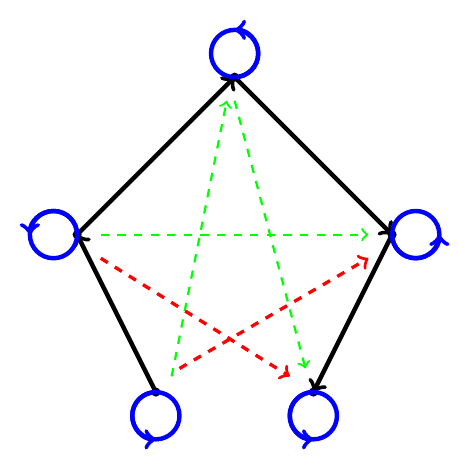
\begin{tikzpicture}[font = \large]
        \draw[ultra thick, ->] (0,0) -- (-1,2);
        \draw[ultra thick, ->] (-1,2) -- (1,4);
        \draw[ultra thick, ->] (1,4) -- (3,2);
        \draw[ultra thick, ->] (3,2) -- (2,0);
        
        \draw[thick, ->, dashed, green] (0.2,0.2) -- (0.9,3.7);
        \draw[thick, ->, dashed, green] (-0.7,2) -- (2.7,2);
        \draw[thick, ->, dashed, green] (1,3.7) -- (1.9,0.3);
        
        \draw[very thick, ->, dashed, red] (0.3,0.3) -- (2.7,1.7);
        \draw[very thick, ->, dashed, red] (-0.7,1.7) -- (1.7,0.2);
        
        \draw [fill = black] (0,0) circle(0.5mm);
        \draw [fill = black] (2,0) circle(0.5mm);
        \draw [fill = black] (3,2) circle(0.5mm);
        \draw [fill = black] (1,4) circle(0.5mm);
        \draw [fill = black] (-1,2) circle(0.5mm);
        
        \draw[ultra thick, blue,rotate = -270] (0,0) arc (360:0:0.3);
        \draw[ultra thick, ->, blue,rotate = -270] (0,0) arc (0:180:0.3);
        
        \draw[ultra thick, blue,rotate = -0] (-1,2) arc (360:0:0.3);
        \draw[ultra thick, ->, blue,rotate = -0] (-1,2) arc (0:180:0.3);
        
        \draw[ultra thick, blue,rotate = -90] (-4,1) arc (360:0:0.3);
        \draw[ultra thick, ->, blue,rotate = -90] (-4,1) arc (0:180:0.3);
        
        \draw[ultra thick, blue,rotate = -180] (-3,-2) arc (360:0:0.3);
        \draw[ultra thick, ->, blue,rotate = -180] (-3,-2) arc (0:180:0.3);
        
        \draw[ultra thick, blue,rotate = -270] (0,-2) arc (360:0:0.3);
        \draw[ultra thick, ->, blue,rotate = -270] (0,-2) arc (0:180:0.3);
        \end{tikzpicture}
\end{figure}

на последнем шаге получится следующий граф:

\begin{figure}[H]
    \centering
    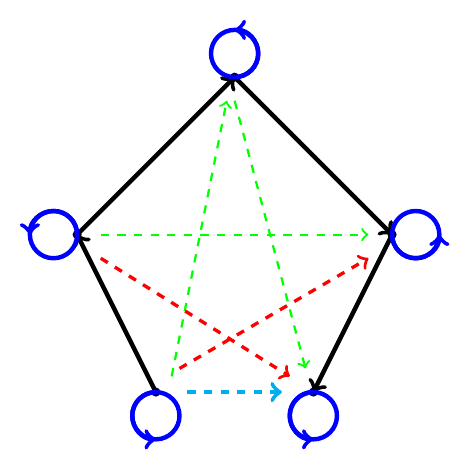
\begin{tikzpicture}[font = \large]
        \draw[ultra thick, ->] (0,0) -- (-1,2);
        \draw[ultra thick, ->] (-1,2) -- (1,4);
        \draw[ultra thick, ->] (1,4) -- (3,2);
        \draw[ultra thick, ->] (3,2) -- (2,0);
        
        \draw[thick, ->, dashed, green] (0.2,0.2) -- (0.9,3.7);
        \draw[thick, ->, dashed, green] (-0.7,2) -- (2.7,2);
        \draw[thick, ->, dashed, green] (1,3.7) -- (1.9,0.3);
        
        \draw[very thick, ->, dashed, red] (0.3,0.3) -- (2.7,1.7);
        \draw[very thick, ->, dashed, red] (-0.7,1.7) -- (1.7,0.2);
        
        \draw[ultra thick, ->, dashed, cyan] (0.4,0) -- (1.6,0);
        
        \draw [fill = black] (0,0) circle(0.5mm);
        \draw [fill = black] (2,0) circle(0.5mm);
        \draw [fill = black] (3,2) circle(0.5mm);
        \draw [fill = black] (1,4) circle(0.5mm);
        \draw [fill = black] (-1,2) circle(0.5mm);
        
        \draw[ultra thick, blue,rotate = -270] (0,0) arc (360:0:0.3);
        \draw[ultra thick, ->, blue,rotate = -270] (0,0) arc (0:180:0.3);
        
        \draw[ultra thick, blue,rotate = -0] (-1,2) arc (360:0:0.3);
        \draw[ultra thick, ->, blue,rotate = -0] (-1,2) arc (0:180:0.3);
        
        \draw[ultra thick, blue,rotate = -90] (-4,1) arc (360:0:0.3);
        \draw[ultra thick, ->, blue,rotate = -90] (-4,1) arc (0:180:0.3);
        
        \draw[ultra thick, blue,rotate = -180] (-3,-2) arc (360:0:0.3);
        \draw[ultra thick, ->, blue,rotate = -180] (-3,-2) arc (0:180:0.3);
        
        \draw[ultra thick, blue,rotate = -270] (0,-2) arc (360:0:0.3);
        \draw[ultra thick, ->, blue,rotate = -270] (0,-2) arc (0:180:0.3);
        \end{tikzpicture}
\end{figure}

\timestamp{16:00}

Можно заметить, что при графе с $5$ вершинами мы сделали $3$ умножения, а при графе с $3$ вершинами мы сделали $1$ умножение. Значит для графа с $n$ вершинами необходимо сделать $n-2$ умножений. 

Теперь мы можем написать алгоритм транзитивного замыкания через умножение матриц.

\timestamp{16:25}
$R$ - матрица отношения.

$R'$ - рефлексивное замыкание $R$. (Добавили петли)
\begin{algorithm}[H]
	\caption{Транзитивное замыкание через умножение матриц}
	\begin{algorithmic}[1]
	    \Statex Инициализация:
	    \State $T := R'$
	    \For{$i$ от $1$ до $n - 2$}
	    \Comment{Цикл с умножением на матрицу отношения}
	        \State $T := T \times R'$
	    \EndFor
	\end{algorithmic}
\end{algorithm}

\timestamp{18:00}
\begin{note}
    $n$ - это размер матрицы (количество вершин в ней).
    
    Когда мы вычисляем один элемент матрицы, мы делаем $n$ умножений, для $n^2$ элементов матрицы нам потребуется сделать $n^3$ операций. Кроме этого есть цикл, выполняемый $n-2$ раза, то есть трудоемкость такого алгоритма будет равна: $C(n)= n \cdot n^2 \cdot (n-2) \approx n^4$.
\end{note}

Существует алгоритм Уоршалла, который позволяет уменьшить трудоемкость алгоритма до $n^3$.

\timestamp{20:50}
\begin{algorithm}[H]
	\caption{Алгоритм транзитивного замыкания Уоршалла}
	\begin{algorithmic}[1]
	    \Statex Инициализация:
	    \State $T := R$
	    \For{$k$ от $1$ до $n$} \Comment{Внешний цикл идет по промежуточным вершинам.}
	        \For{$i$ от $1$ до $n$} \Comment{Циклы по $i$ и $j$ перебирают всевозможные пары.}
    	        \For{$j$ от $1$ до $n$}
    	            \State $T(i;j)$ := $max$ \{$T(i;j) , \ T(i;k) \cdot T(k;j)\}$ \Comment{Благодаря операции $max$ сохраняются те связи, которые были.}
    	        \EndFor
	    \EndFor
	    \EndFor
	\end{algorithmic}
\end{algorithm}

\begin{note}
    Трудоемкость такого алгоритма будет $n^3$.
    
    Важно понимать, что цикл по $k$ нельзя поменять с другими циклами: алгоритм в таком случае правильно работать не будет. При этом циклы по $i$ и $j$ местами менять можно. Смысл основной операции в теле цикла
    $T(i;j)$ := $max$ \{$T(i;j) , \ T(i;k) \cdot T(k;j)\}$ состоит в том, что если $i$ и $j$ уже находятся в отношении, то соответствующий элемент $T(i;j)$ не меняется, иначе ищем, нет ли элемента $k$, находящегося в отношении с элементами $i$ и $j$, то есть элемента $k$ такого, что $T(i; k)=1$ и $T(k; j)=1$, тогда  $T(i; k) \cdot T(k; j) = 1$, и мы добавляем отношение между $i$ и $j$, то есть полагаем $T(i;j)=1$. Доказательство корректности алгоритма основано на том, что на каждом шаге внешнего цикла расширяется число промежуточных вершин в путях между вершинами. Аккуратное доказательство будет дано позже при рассмотрении алгоритма Флойда, который обобщает алгоритм Уоршалла
\end{note}
         
\newpage

\timestamp{26:40}

\section{Эйлеровы графы}

\begin{definition}
    Мультиграфом (псевдографом, когда есть петли) называется граф, в котором две вершины могут быть соединены более чем одним ребром.
\end{definition}

Для начала введем понятие уникурсальной кривой, смысл которой заключается в том, что ее можно нарисовать, не отрывая руки.

Обратимся к задачам, в которых требуется нарисовать фигуры, не отрывая от руки. 

Сначала предлагают открытый конверт,

\timestamp{28:20}
\begin{figure}[H]
    \centering
    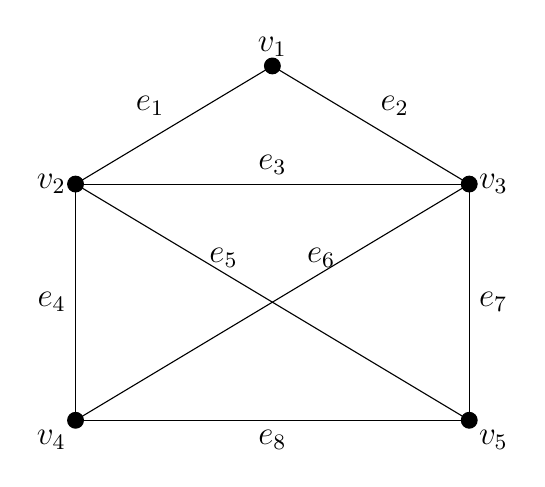
\begin{tikzpicture}[font = \large]
        \draw 
        (0,3) -- node[above]{$e_3$}
        (5,3) -- node[]{} cycle;
        
        \draw 
        (5,3) -- node[right]{$e_7$}
        (5,0) -- node[]{} cycle;
        
        \draw 
        (0,0) -- node[below]{$e_8$}
        (5,0) -- node[]{} cycle;
        
        \draw 
        (0,0) -- node[left]{$e_4$}
        (0,3) -- node[]{} cycle;
        
        \draw 
        (5,0) -- node[above right = 9pt]{$e_6$}
        (0,3) -- node[]{} cycle;
        
        \draw 
        (0,0) -- node[above left = 9pt]{$e_5$}
        (5,3) -- node[]{} cycle;
        
        \draw 
        (0,3) -- node[above left]{$e_1$}
        (2.5,4.5) -- node[]{} cycle;
        
        \draw 
        (2.5,4.5) -- node[above right]{$e_2$}
        (5,3) -- node[]{} cycle;
        
        \draw [fill = black] (0,0) circle(1mm) node[below left]{$v_4$};
        \draw [fill = black] (5,0) circle(1mm) node[below right]{$v_5$};
        \draw [fill = black] (5,3) circle(1mm) node[right]{$v_3$};
        \draw [fill = black] (0,3) circle(1mm) node[left]{$v_2$};
        \draw [fill = black] (2.5,4.5) circle(1mm) node[above]{$v_1$};
    \end{tikzpicture}
    \label{pic:7}
\end{figure}

а затем закрытый.

\begin{figure}[H]
    \centering
    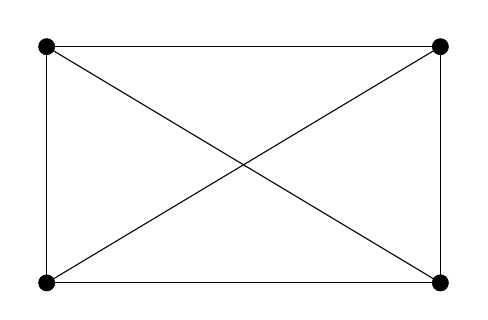
\begin{tikzpicture}[font = \large]
        \draw 
        (0,3) -- node[above]{}
        (5,3) -- node[]{} cycle;
        
        \draw 
        (5,3) -- node[right]{}
        (5,0) -- node[]{} cycle;
        
        \draw 
        (0,0) -- node[above]{}
        (5,0) -- node[]{} cycle;
        
        \draw 
        (0,0) -- node[left]{}
        (0,3) -- node[]{} cycle;
        
        \draw 
        (5,0) -- node[above right = 9pt]{}
        (0,3) -- node[]{} cycle;
        
        \draw 
        (0,0) -- node[above left = 9pt]{}
        (5,3) -- node[]{} cycle;
        
        \draw [fill = black] (0,0) circle(1mm);
        \draw [fill = black] (5,0) circle(1mm);
        \draw [fill = black] (5,3) circle(1mm);
        \draw [fill = black] (0,3) circle(1mm);
    \end{tikzpicture}
\end{figure}

Открытый конверт можно нарисовать, не отрывая руки, в отличие от закрытого. Графы, которые можно нарисовать, не отрывая руки, называют эйлеровыми.

\timestamp{30:35}
\begin{definition}
    Путь в графе - это последовательность вершин и ребер, при этом обязательно каждое ребро, находящееся между вершинами, соединяет эти вершины.
\end{definition}

Путь, по которому можно нарисовать открытый конверт, не отрывая руки: 

$v_5 e_8 v_4 e_4 v_2 e_5 v_5 e_7 v_3 e_3 v_2 e_1 v_1 e_2 v_3 e_6 v_4$

Заметим, что в "обычном" графе - не мультиграфе - путь, проходящий через каждое ребро не более чем по одному разу, можно определить как последовательность вершин, через которые он проходит (такие пути называются простыми), например, для открытого конверта это будет $v_5 v_4 v_2 v_5 v_3 v_2 v_1 v_3 v_4$.

\timestamp{32:50}
\begin{definition}
    Эйлеров путь в графе - это путь, который проходит по всем ребрам графа (граф, в таком случае, является связным) и при этом только один раз через каждое ребро.
\end{definition}

\begin{note}
    Если конечная точка эйлерова пути совпадает с начальной, то его называют \emph{эйлеровым циклом}.
\end{note}

Также есть понятие гамильтонова пути, когда каждая вершина графа встречается в нем ровно один раз, и все вершины графа входят в этот путь, Заметим, что гамильтонов путь не обязательно содержит все ребра. Можно рассматривать гамильтонов цикл, в котором совпадает начальная и конечная вершины.

Следует обратить внимание на то, что если в графе, изображающем открытый конверт, добавить ребро, которое соединяет вершины $v_4$ и $v_5$, и включить его в путь, то в получившемся мультиграфе будет построен эйлеров цикл

\timestamp{33:55}

\begin{figure}[H]
    \centering
    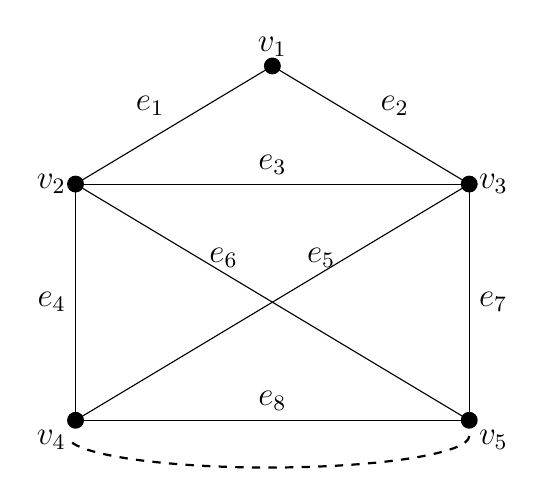
\begin{tikzpicture}[font = \large]
        \draw 
        (0,3) -- node[above]{$e_3$}
        (5,3) -- node[]{} cycle;
        
        \draw 
        (5,3) -- node[right]{$e_7$}
        (5,0) -- node[]{} cycle;
        
        \draw 
        (0,0) -- node[above]{$e_8$}
        (5,0) -- node[]{} cycle;
        
        \draw 
        (0,0) -- node[left]{$e_4$}
        (0,3) -- node[]{} cycle;
        
        \draw 
        (5,0) -- node[above right = 9pt]{$e_5$}
        (0,3) -- node[]{} cycle;
        
        \draw 
        (0,0) -- node[above left = 9pt]{$e_6$}
        (5,3) -- node[]{} cycle;
        
        \draw 
        (0,3) -- node[above left]{$e_1$}
        (2.5,4.5) -- node[]{} cycle;
        
        \draw 
        (2.5,4.5) -- node[above right]{$e_2$}
        (5,3) -- node[]{} cycle;
        
        \draw [fill = black] (0,0) circle(1mm) node[below left]{$v_4$};
        \draw [fill = black] (5,0) circle(1mm) node[below right]{$v_5$};
        \draw [fill = black] (5,3) circle(1mm) node[right]{$v_3$};
        \draw [fill = black] (0,3) circle(1mm) node[left]{$v_2$};
        \draw [fill = black] (2.5,4.5) circle(1mm) node[above]{$v_1$};
        
        \draw [thick, dashed] (5,-0.2) arc (0:-180:2.55 and 0.4);
    \end{tikzpicture}
\end{figure}

Поэтому задачу на нахождение эйлеровых путей и эйлеровых циклов можно свести одну к другой.

\timestamp{34:30}
Если в графе построен эйлеров цикл, то в каждой вершине сходится четное число ребер, так как по одному ребру мы "входим" в вершину, по другому "выходим".

\timestamp{35:25}
\begin{definition}
    Степень вершины - это количество количество концов ребер, сходящихся в этой вершине. Такое отношение между ребром и вершиной будем называть инцидентностью.
\end{definition}

\timestamp{35:05}
\begin{example}
    Если $v_{1},v_{2}$ — вершины, а $e_1=(v_{1},v_{2})$ — соединяющее их ребро, тогда вершина $v_{1}$ и ребро $e$ инцидентны, вершина $v_{2}$ и ребро $e_1$ тоже инцидентны.
\end{example}

\begin{note}
    Если граф ориентированный, то иногда количество входящих и выходящих из вершины рёбер считают отдельно и говорят о положительной или выходной и отрицательной или входной степенях вершины.
\end{note}

\timestamp{36:00}
Из рассмотренных определений непосредственно следует необходимое условие существования эйлерового цикла: четность степеней вершин графа. 

\timestamp{37:20} 
Рассмотрим следующий двухкомпонентный граф, чтобы узнать, является ли это условие достаточным.

\begin{figure}[H]
    \centering
    \begin{tikzpicture}[font = \large, scale = 0.7]
        \draw (0,0) -- (3,0) -- (3,3) -- (0,3) -- cycle;
        
        \draw (4,0) -- (7,0) -- (5.5,3) -- cycle;
    \end{tikzpicture}    
\end{figure}

Данный граф невозможно нарисовать, не отрывая руки, хотя все степени вершин четные.

\begin{definition}
    Связный граф — граф, между любыми двумя вершинами которого существует соединяющий их путь. Если же граф не связан, то можно найти две вершины, между которыми такого пути нет. 
\end{definition}

Таким образом необходимо добавить еще одно условие - условие связности графа, чтобы получить необходимое и достаточное условие эйлеровости графа.

\timestamp{38:20}
\begin{theorem}[Об эйлеровых графах]
Связный неориентированный граф является эйлеровым, когда либо все вершины имеют четную степень, либо все кроме двух.
\end{theorem}

\begin{note}
    В первом случае будет эйлеров цикл, а во втором эйлеров путь.
\end{note}

\timestamp{40:00}
Мы уже доказали, что если есть такой цикл, то все вершины имеют четную степень, теперь докажем, что мы всегда сможем обойти граф, обладающий таким свойством.

Рассмотрим следующий граф:

\begin{figure}[H]
    \centering
    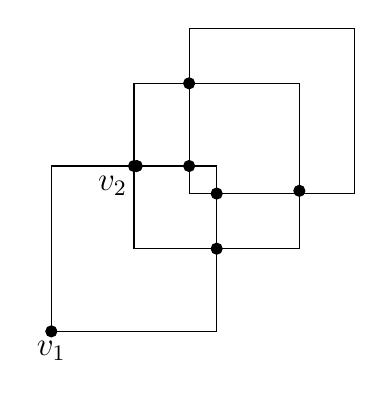
\begin{tikzpicture}[font = \large, scale = 0.7]
        \draw (0,0) -- (3,0) -- (3,3) -- (0,3) -- cycle;
        
        \draw (1.5,1.5) -- (4.5,1.5);
        \draw (4.5,1.5) -- (4.5,4.5);
        \draw (4.5,4.5) -- (1.5,4.5);
        \draw (1.5,1.5) -- (1.5,4.5);
        
        \draw (2.5,2.5) -- (5.5,2.5);
        \draw (5.5,2.5) -- (5.5,5.5);
        \draw (5.5,5.5) -- (2.5,5.5);
        \draw (2.5,2.5) -- (2.5,5.5);
        
        \draw [fill = black] (1.5,3) circle(1mm);
        \draw [fill = black] (3,1.5) circle(1mm);
        \draw [fill = black] (2.5,3) circle(1mm);
        \draw [fill = black] (3,2.5) circle(1mm);
        \draw [fill = black] (2.5,4.5) circle(1mm);
        \draw [fill = black] (4.5,2.55) circle(1mm);
        
        \draw [fill = black] (0,0) circle(1mm) node[below]{$v_1$};
        \draw [fill = black] (1.55,3) circle(1mm) node[below left]{$v_2$};
    \end{tikzpicture}
\end{figure}

Данный граф надо обвести, не отрывая руки.

\timestamp{40:30}
Начнем с любой вершины, допустим с $v_1$. Поскольку все вершины четные, то при входе в какую-либо веришну необходимо из нее выйти. 

Допустим, что мы пошли неправильно и вернулись в начало, найдя цикл, который не является эйлеровым. Значит есть еще вершины, для которых пройдены не все инцидентные им ребра.

\begin{figure}[H]
    \centering
    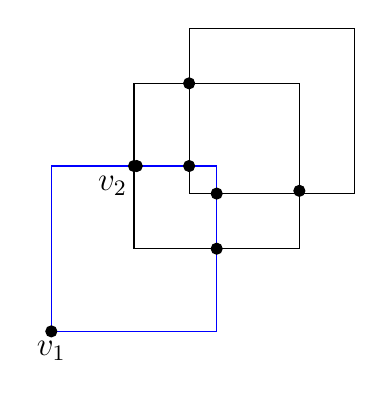
\begin{tikzpicture}[font = \large, scale = 0.7]
        \draw[blue] (0,0) -- (3,0) -- (3,3) -- (0,3) -- cycle;
        
        \draw (1.5,1.5) -- (4.5,1.5);
        \draw (4.5,1.5) -- (4.5,4.5);
        \draw (4.5,4.5) -- (1.5,4.5);
        \draw (1.5,1.5) -- (1.5,4.5);
        
        \draw (2.5,2.5) -- (5.5,2.5);
        \draw (5.5,2.5) -- (5.5,5.5);
        \draw (5.5,5.5) -- (2.5,5.5);
        \draw (2.5,2.5) -- (2.5,5.5);
        
        \draw [fill = black] (1.5,3) circle(1mm);
        \draw [fill = black] (3,1.5) circle(1mm);
        \draw [fill = black] (2.5,3) circle(1mm);
        \draw [fill = black] (3,2.5) circle(1mm);
        \draw [fill = black] (2.5,4.5) circle(1mm);
        \draw [fill = black] (4.5,2.55) circle(1mm);
        
        \draw [fill = black] (0,0) circle(1mm) node[below]{$v_1$};
        \draw [fill = black] (1.55,3) circle(1mm) node[below left]{$v_2$};
    \end{tikzpicture}
\end{figure}

\begin{note}
    Синим обозначен цикл, который мы нашли.
\end{note}

Берем первую из таких вершин $v_2$ и опять начинаем идти, пока не дойдем до того места, откуда вышли. Зайти "в тупик" не получится, так как в каждой вершине графа, куда можно попасть есть четное число непройденных ребер.
Если мы обошли все ребра, то необходимо путь из $v_2$ склеить с путем из $v_1$. Если полученный путь не будет эйлеровым, то нужно повторить процедуру наращивания пути.

\begin{figure}[H]
    \centering
    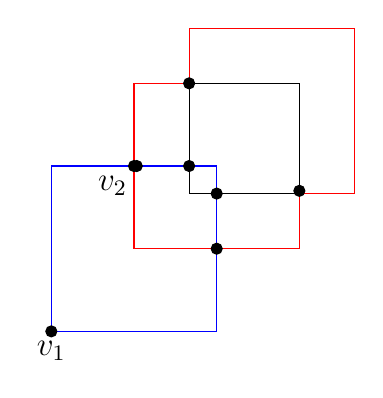
\begin{tikzpicture}[font = \large, scale = 0.7]
        \draw [blue] (0,0) -- (3,0) -- (3,3) -- (0,3) -- cycle;
        
        \draw (1.5,1.5) -- (4.5,1.5);
        \draw (4.5,1.5) -- (4.5,4.5);
        \draw (4.5,4.5) -- (1.5,4.5);
        \draw (1.5,1.5) -- (1.5,4.5);
        
        \draw (2.5,2.5) -- (5.5,2.5);
        \draw (5.5,2.5) -- (5.5,5.5);
        \draw (5.5,5.5) -- (2.5,5.5);
        \draw (2.5,2.5) -- (2.5,5.5);
        
        \draw [red] (1.5,3) -- (1.5,4.5) -- (2.5,4.5) -- (2.5,5.5) -- (5.5,5.5) -- (5.5,2.5) -- (4.5,2.5) -- (4.5,1.5) -- (3,1.5) -- (1.5,1.5)-- cycle;
        
        \draw [fill = black] (1.5,3) circle(1mm);
        \draw [fill = black] (3,1.5) circle(1mm);
        \draw [fill = black] (2.5,3) circle(1mm);
        \draw [fill = black] (3,2.5) circle(1mm);
        \draw [fill = black] (2.5,4.5) circle(1mm);
        \draw [fill = black] (4.5,2.55) circle(1mm);
        
        \draw [fill = black] (0,0) circle(1mm) node[below]{$v_1$};
        \draw [fill = black] (1.55,3) circle(1mm) node[below left]{$v_2$};
    \end{tikzpicture}
\end{figure}

\timestamp{42:30}
В приведенном методе не описано, как быстро находить вершины с непройденными ребрами. Использование стека позволяет превратить описанный метод в эффективный алгоритм. Найдите этот алгоритм и реализуйте его.

\newpage

\timestamp{43:00}

\section{Теорема Эйлера}

Перейдем к изучению циклов графа. Оказывается, что их можно некоторым образом складывать (и умножать на $1$ или $0$), получая другие циклы, и по этим операциям циклы образуют линейное пространство.

\timestamp{45:15}
Рассмотрим следующий граф, в котором требуется найти все циклы:
\begin{figure}[H]
    \centering
    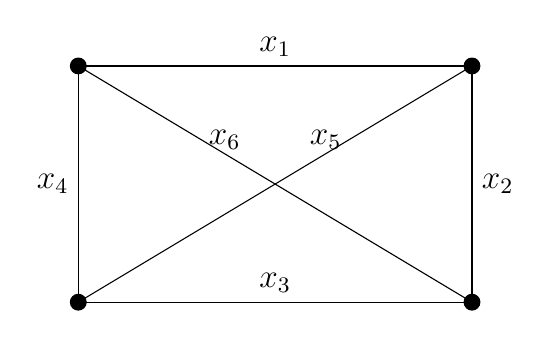
\begin{tikzpicture}[font = \large]
        \draw 
        (0,3) -- node[above]{$x_1$}
        (5,3) -- node[]{} cycle;
        
        \draw 
        (5,3) -- node[right]{$x_2$}
        (5,0) -- node[]{} cycle;
        
        \draw 
        (0,0) -- node[above]{$x_3$}
        (5,0) -- node[]{} cycle;
        
        \draw 
        (0,0) -- node[left]{$x_4$}
        (0,3) -- node[]{} cycle;
        
        \draw 
        (5,0) -- node[above right = 9pt]{$x_5$}
        (0,3) -- node[]{} cycle;
        
        \draw 
        (0,0) -- node[above left = 9pt]{$x_6$}
        (5,3) -- node[]{} cycle;
        
        \draw [fill = black] (0,0) circle(1mm);
        \draw [fill = black] (5,0) circle(1mm);
        \draw [fill = black] (5,3) circle(1mm);
        \draw [fill = black] (0,3) circle(1mm);
    \end{tikzpicture}
    \label{pic:8}
\end{figure}

Каждому ребру мы сопоставим переменную $(x_1,\dotsc,x_6)$, значение которой будет равно либо $1$ (включаем ребро графа в цикл), либо $0$ (не включаем).

Каждой вершине мы сопоставим уравнение, основанное на свойстве цикла - каждой вершине циклического пути инцидентно четное число ребер. В терминах введенных переменных это означает, что сумма переменных, соответствующих инцидентным вершине ребрам, равна $0$ по модулю $2$.

\systeme{
x_1 + x_4 + x_5 = 0,
x_1 + x_2 + x_6 = 0,
x_3 + x_4 + x_6 = 0,
x_2 + x_3 + x_5 = 0}

\begin{note}
    Система уравнений рассматривается в $\mathbb{Z}_2$ - арифметике вычетов по модулю $2$.
\end{note}

\timestamp{48:45}
Решим данную систему уравнений:

\noindent
$\begin{pmatrix}
  1 & 0 & 0 & 1 & 1 & 0\\
  1 & 1 & 0 & 0 & 0 & 1\\
  0 & 0 & 1 & 1 & 0 & 1\\
  0 & 1 & 1 & 0 & 1 & 0\\
  \end{pmatrix}
  \rightarrow
  \begin{pmatrix}
  1 & 0 & 0 & 1 & 1 & 0\\
  0 & 1 & 0 & 1 & 1 & 1\\
  0 & 0 & 1 & 1 & 0 & 1\\
  0 & 1 & 1 & 0 & 1 & 0\\
  \end{pmatrix}
  \rightarrow
  \begin{pmatrix}
  1 & 0 & 0 & 1 & 1 & 0\\
  0 & 1 & 0 & 1 & 1 & 1\\
  0 & 0 & 1 & 1 & 0 & 1\\
  0 & 0 & 1 & 1 & 1 & 1\\
  \end{pmatrix}
  \rightarrow
  \\
  \\
  \begin{pmatrix}
  1 & 0 & 0 & 1 & 1 & 0\\
  0 & 1 & 0 & 1 & 1 & 1\\
  0 & 0 & 1 & 1 & 0 & 1\\
  0 & 0 & 0 & 0 & 0 & 0\\
\end{pmatrix}
$
\timestamp{51:00}
\begin{note}
    Заметим, что если есть одна компонента связности, то обязательно последняя строка в матрице всегда будет нулевой. Если компонент связности две, то, аналогично, исчезнет два уравнения. Причины этого обсудим позже.
\end{note}

\timestamp{52:30}

Запишем множество решений в параметрическом виде, для чего трем последним переменным позволим принимать произвольные значения (таких значений всего два: $0$ и $1$) и обозначим их параметрами $t$ с соответствующими индексами. В матричном представлении это означает рассмотрение расширенной матрицы. Заметим что перенос членов уравнения в правую часть не требует изменения знака, так как в арифметике вычетов по модулю два $1 = -1$


$\left(  
\begin{tabular}{ccc|ccc}
$x_1$ & $x_2$ & $x_3$ & $t_1$ & $t_2$ & $t_3$ \\
1 & 0 & 0 & 1 & 1 & 0 \\
0 & 1 & 0 & 1 & 1 & 1 \\
0 & 0 & 1 & 1 & 0 & 1 \\
0 & 0 & 0 & 0 & 0 & 0
\end{tabular}
\right)
$
$\rightarrow$
\systeme{
x_1 = t_1 + t_2,
x_2 = t_1 + t_2 + t_3,
x_3= t_1 + t_3,}

откуда:

\timestamp{54:10}
Весь вектор решений можно переписать в виде пространства решений:
$$\begin{pmatrix}
  x_1\\
  x_2\\
  x_3\\
  x_4\\
  x_5\\
  x_6\\
\end{pmatrix}
=
\begin{pmatrix}
  t_1+t_2\\
  t_1+t_2+t_3\\
  t_1+t_3\\
  t_1\\
  t_2\\
  t_3\\
\end{pmatrix}
$$

\begin{note}
    Если бы операции выполнялись с вещественными числами, то мы бы получили бесконечное множество решений, однако в нашем случае $t_1, t_2, t_3$ равны либо $0$, либо $1$, поэтому это множество содержит всего $8$ решений, причем одно из них - нулевое - не соответствует никакому циклу, так что невырожденных решений $7$. Это хорошо видно из следующего разложения.
\end{note}

\timestamp{54:45}

Разложим полученный вектор на базисные циклы.
$$
\begin{pmatrix}
  t_1+t_2\\
  t_1+t_2+t_3\\
  t_1+t_3\\
  t_1\\
  t_2\\
  t_3\\
\end{pmatrix} 
=
\begin{pmatrix}
  1\\
  1\\
  1\\
  1\\
  0\\
  0\\
\end{pmatrix}
t_1
+
\begin{pmatrix}
  1\\
  1\\
  0\\
  0\\
  1\\
  0\\
\end{pmatrix}
t_2
+
\begin{pmatrix}
  0\\
  1\\
  1\\
  0\\
  0\\
  1\\
\end{pmatrix}
t_3
$$

\begin{note}
    Вектора в правой части соответствуют следующим циклам графа:
    
    \begin{figure}[h]
    \begin{minipage}[h]{0.15\linewidth}
    \begin{figure}[H]
    \centering
        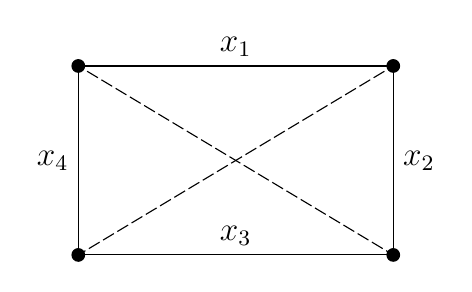
\begin{tikzpicture}[font = \large, scale = 0.8]
            \draw 
            (0,3) -- node[above]{$x_1$}
            (5,3) -- node[]{} cycle;
            
            \draw 
            (5,3) -- node[right]{$x_2$}
            (5,0) -- node[]{} cycle;
            
            \draw 
            (0,0) -- node[above]{$x_3$}
            (5,0) -- node[]{} cycle;
            
            \draw 
            (0,0) -- node[left]{$x_4$}
            (0,3) -- node[]{} cycle;
            
            \draw [dashed]
            (5,0) -- node[above right = 9pt]{}
            (0,3) -- node[]{} cycle;
            
            \draw [dashed]
            (0,0) -- node[above left = 9pt]{}
            (5,3) -- node[]{} cycle;
            
            \draw [fill = black] (0,0) circle(1mm);
            \draw [fill = black] (5,0) circle(1mm);
            \draw [fill = black] (5,3) circle(1mm);
            \draw [fill = black] (0,3) circle(1mm);
        \end{tikzpicture}
    \end{figure}
    \end{minipage}
    \hfill
    \begin{minipage}[h]{0.15\linewidth}
        \begin{figure}[H]
        \centering
        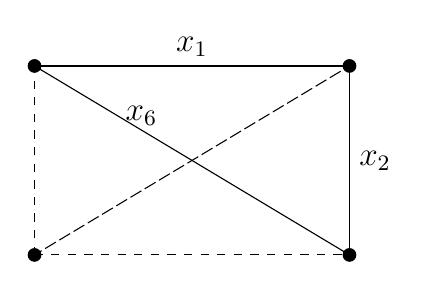
\begin{tikzpicture}[font = \large, scale = 0.8]
            \draw 
            (0,3) -- node[above]{$x_1$}
            (5,3) -- node[]{} cycle;
            
            \draw 
            (5,3) -- node[right]{$x_2$}
            (5,0) -- node[]{} cycle;
            
            \draw [dashed]
            (0,0) -- (5,0);
            
            \draw [dashed]
            (0,0) -- (0,3);
            
            \draw 
            (5,0) -- node[above right = 9pt]{}
            (0,3) -- node[]{} cycle;
            
            \draw [dashed]
            (0,0) -- node[above left = 9pt]{$x_6$}
            (5,3) -- node[]{} cycle;
            
            \draw [fill = black] (0,0) circle(1mm);
            \draw [fill = black] (5,0) circle(1mm);
            \draw [fill = black] (5,3) circle(1mm);
            \draw [fill = black] (0,3) circle(1mm);
        \end{tikzpicture}
    \end{figure}
    \end{minipage}
    \hfill
    \begin{minipage}[h]{0.15\linewidth}
    \begin{figure}[H]
    \centering
        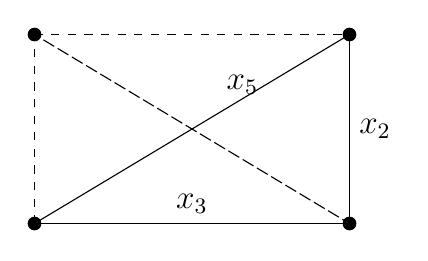
\begin{tikzpicture}[font = \large, scale = 0.8]
            \draw [dashed]
            (0,3) -- 
            (5,3);
            
            \draw 
            (5,3) -- node[right]{$x_2$}
            (5,0) -- node[]{} cycle;
            
            \draw 
            (0,0) -- node[above]{$x_3$}
            (5,0) -- node[]{} cycle;
            
            \draw [dashed]
            (0,0) -- 
            (0,3);
            
            \draw [dashed]
            (5,0) -- node[above right = 9pt]{$x_5$}
            (0,3) -- node[]{} cycle;
            
            \draw 
            (0,0) -- node[above left = 9pt]{}
            (5,3) -- node[]{} cycle;
            
            \draw [fill = black] (0,0) circle(1mm);
            \draw [fill = black] (5,0) circle(1mm);
            \draw [fill = black] (5,3) circle(1mm);
            \draw [fill = black] (0,3) circle(1mm);
        \end{tikzpicture}
    \end{figure}
    \end{minipage}
    \end{figure}

\end{note}

\timestamp{57:00}
\begin{example}
    Если мы присвоим $t_1$ и $t_2$ значение $1$, а $t_3$ $0$, то получится следующий цикл:
    
$
\begin{pmatrix}
  1\\
  1\\
  1\\
  1\\
  0\\
  0\\
\end{pmatrix}
t_1
+
\begin{pmatrix}
  1\\
  1\\
  0\\
  0\\
  1\\
  0\\
\end{pmatrix}
t_2
=
$
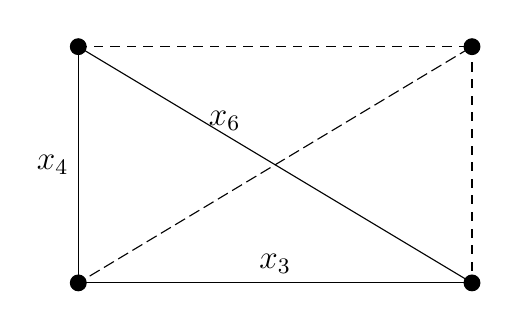
\begin{tikzpicture}[font = \large]
    \draw [dashed]
    (0,3) -- node[above]{}
    (5,3) -- node[]{} cycle;
    
    \draw [dashed]
    (5,3) -- node[right]{}
    (5,0) -- node[]{} cycle;
    
    \draw 
    (0,0) -- node[above]{$x_3$}
    (5,0) -- node[]{} cycle;
    
    \draw 
    (0,0) -- node[left]{$x_4$}
    (0,3) -- node[]{} cycle;
    
    \draw
    (5,0) -- node[above right = 9pt]{}
    (0,3) -- node[]{} cycle;
    
    \draw [dashed]
    (0,0) -- node[above left = 9pt]{$x_6$}
    (5,3) -- node[]{} cycle;
    
    \draw [fill = black] (0,0) circle(1mm);
    \draw [fill = black] (5,0) circle(1mm);
    \draw [fill = black] (5,3) circle(1mm);
    \draw [fill = black] (0,3) circle(1mm);
\end{tikzpicture}
\end{example}

\newpage
\timestamp{58:25}
Рассмотрим систему уравнений для описания пространства циклов в общем виде. Схематично матрица системы выглядит так:
\begin{figure}[H]
    \centering
    \includegraphics[width=4cm, height=4cm]{9.1.png}
\end{figure}

\begin{itemize}
    \item Количество уравнений \emph{B} равно количеству вершин в графе. 
    \item Количество переменных \emph{Р} равно количеству рёбер в рафе.
    \item Количество нулевых строчек, после применения к матрице алгоритма Гаусса, равно числу компонент связности  \emph{К}.
\end{itemize}

Докажем, что сумма уравнений для вершин из одной компоненты связности равна 0, то есть они линейно зависимы и одно уравнение можно убрать (или заменить строку в матрице строкой нулей). Действительно, каждая переменная, соответствующая ребру, будет фигурировать в этих уравнениях дважды: один раз в уравнении, сопоставленном одному концу ребра, второй раз - другому. Тогда при сложении уравнений по модулю два коэффициенты при всех переменных будут равны нулю. Объясним на следующем примере, что для уравнений, не образующих компоненту связности, линейной зависимости не будет.

\begin{figure}[H]
    \centering
    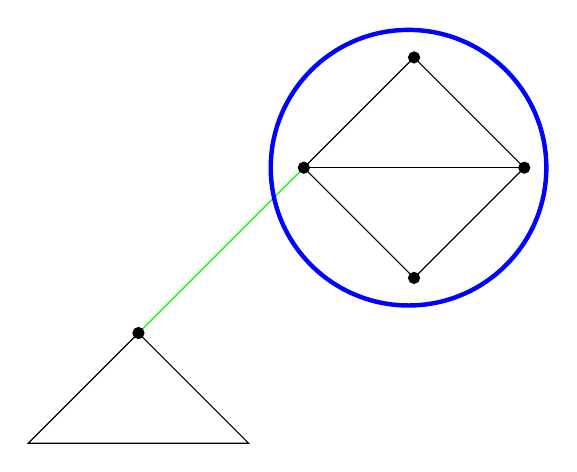
\begin{tikzpicture}[font = \large, scale = 0.7]
        \draw (0,0) -- (4,0) -- (2,2) -- cycle;
        
        \draw (7,7) -- (5,5) -- (7,3) -- (9,5) -- cycle;
        
        \draw (5,5) -- (9,5);
        \draw [green] (2,2) -- (5,5);
        
        \draw [fill = black] (2,2) circle(1mm);
        \draw [fill = black] (7,7) circle(1mm);
        \draw [fill = black] (5,5) circle(1mm);
        \draw [fill = black] (7,3) circle(1mm);
        \draw [fill = black] (9,5) circle(1mm);
        \draw [ultra thick, blue] (9.4,5) arc (360:0:2.5);
\end{tikzpicture}
\end{figure}

Заметим, что вершина, инцидентная зеленому ребру (выходящему за пределы круга), будет учтена в уравнениях, соответствующих вершинам внутри круга, только один раз. Поэтому сумма этих уравнений не будет равна нулю (переменная, соответствующая зеленому ребру останется). Тем самым утверждение доказано.

\timestamp{1:01:05}
Таким образом, применение метода Гаусса позволяет привести систему к стандартной трапециевидной форме (пунктиром обозначена диагональная или треугольная матрица), где в правой части находятся наши параметры. Ц - число параметров - является размерностью нашего пространства (числом независимых циклов).
\begin{figure}[H]
    \centering
    \includegraphics[width=4cm, height=4cm]{9.2.png}
\end{figure}

Так как область с пунктирной линией является квадратом, то  В - К это длина одной стороны квадрата, а Р - Ц - другой, поэтому они равны. Отсюда получаем формулу Эйлера:

\begin{equation*}
    \text{В - К = Р - Ц}
    \label{eq:Eyler}
\end{equation*}

\begin{note}
    Данную формулу чаще записывают в следующем виде $$\text{В + Ц = Р + К}$$
\end{note}

\begin{note}

\timestamp{1:02:35}
Существует более простой способ найти число независимых циклов, который позволяет не решать систему уравнений.

\begin{definition}
    Остовное дерево — связный подграф (часть графа) данного связного неориентированного графа, который включает все его вершины и при этом в нем нет циклов.
\end{definition}

\begin{figure}[H]
    \centering
    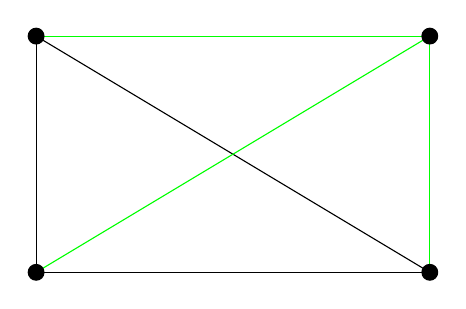
\begin{tikzpicture}[font = \large]
        \draw [green]
        (0,3) -- (5,3);
        
        \draw [green]
        (5,3) -- (5,0);
        
        \draw 
        (0,0) -- (5,0);
        
        \draw 
        (0,0) -- (0,3);
        
        \draw
        (5,0) -- (0,3);
        
        \draw [green]
        (0,0) -- (5,3);
        
        \draw [fill = black] (0,0) circle(1mm);
        \draw [fill = black] (5,0) circle(1mm);
        \draw [fill = black] (5,3) circle(1mm);
        \draw [fill = black] (0,3) circle(1mm);
    \end{tikzpicture}
\end{figure}

\begin{note}
    Зелёным цветом обозначено остовное дерево.
\end{note}

Количество рёбер, которые не входят в остовное дерево, будет равно числу независимых циклов. Поочередное добавление ребер, не входящих в остовное дерево, будет давать все циклы базиса пространства циклов.

\begin{note}
    Если выбрать другое остовное дерево, получим другой базис пространства циклов.
\end{note}

\begin{problem}
    Напишите программу построения базиса пространства циклов, основанную на этой идее.
\end{problem}

\end{note}

\timestamp{1:03:55}
Далее рассмотрим как формула Эйлера применяется для многогранников и плоских графов (графов, изображенных на плоскости без пересечения ребер).

\begin{figure}[H]
    \centering
    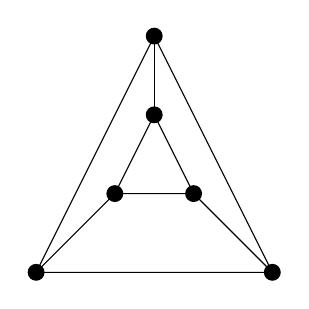
\begin{tikzpicture}[]
            \draw (0,0) -- (1,0) -- (0.5,1)  -- cycle;
            
            \draw (-1,-1) -- (2,-1) -- (0.5,2)  -- cycle;
            
            \draw (-1,-1) -- (0,0);
            \draw (2,-1) -- (1,0);
            \draw (0.5,2) -- (0.5,1);
            
            \draw [fill = black] (0,0) circle(1mm);
            \draw [fill = black] (1,0) circle(1mm);
            \draw [fill = black] (0.5,1) circle(1mm);
            \draw [fill = black] (-1,-1) circle(1mm);
            \draw [fill = black] (2,-1) circle(1mm);
            \draw [fill = black] (0.5,2) circle(1mm);
    \end{tikzpicture}
    \caption{Пример плоского графа}
\end{figure}

\begin{note}
    Данный граф может быть нарисован так, что у него будут пересечения ребер, но перемещением вершин по плоскости можно достичь того, что пересечений не будет, то есть, он станет плоским. Такой "потенциально плоский" \ граф называется планарным.
\end{note}

\begin{figure}[H]
    \centering
     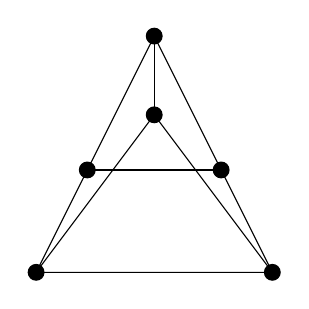
\begin{tikzpicture}
             \draw (-0.35,0.3)  -- (1.35,0.3) -- cycle;
        
            \draw (-1,-1) -- (2,-1) -- (0.5,2)  -- cycle;
            
            \draw (-1,-1) -- (0.5,1);
            \draw (2,-1) -- (0.5,1);
            \draw (0.5,2) -- (0.5,1);
            
            \draw [fill = black] (-0.35,0.3) circle(1mm);
            \draw [fill = black] (1.35,0.3) circle(1mm);
            \draw [fill = black] (0.5,1) circle(1mm);
            \draw [fill = black] (-1,-1) circle(1mm);
            \draw [fill = black] (2,-1) circle(1mm);
            \draw [fill = black] (0.5,2) circle(1mm);
     \end{tikzpicture}
    \caption{Пример планарного графа}
\end{figure}

Если граф плоский, то все области ($G_1,G_2,G_3,G_4,G_5$), на которые он делит плоскость, называются гранями.

\begin{figure}[H]
    \centering
    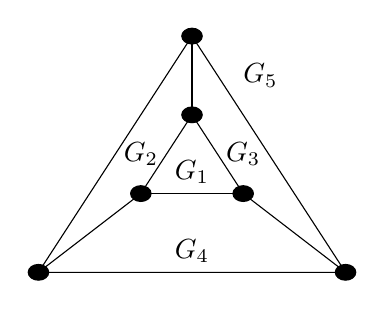
\begin{tikzpicture}[xscale = 1.3]
            \draw 
            (0,0) -- node[above]{$G_1$}
            (1,0) -- node[]{} cycle;
            \draw
            (1,0) -- node[left = 18pt]{$G_2$}
            (0.5,1) -- node[]{} cycle;
            \draw
            (0.5,1) -- node[right = 18pt]{$G_3$}
            (0,0) -- node[]{} cycle;
            
            \draw
            (-1,-1) -- node[above]{$G_4$}
            (2,-1) -- node[]{} cycle;
            
            \draw (0.5,2) -- node[right = 15pt]{$G_5$}
            (0.5,1) -- node[]{} cycle;
            
            \draw (-1,-1) -- (2,-1) -- (0.5,2)  -- cycle;
            
            \draw (-1,-1) -- (0,0);
            \draw (2,-1) -- (1,0);
            \draw (0.5,2) -- (0.5,1);
            
            \draw [fill = black] (0,0) circle(1mm);
            \draw [fill = black] (1,0) circle(1mm);
            \draw [fill = black] (0.5,1) circle(1mm);
            \draw [fill = black] (-1,-1) circle(1mm);
            \draw [fill = black] (2,-1) circle(1mm);
            \draw [fill = black] (0.5,2) circle(1mm);
    \end{tikzpicture}
\end{figure}

\begin{example}
    Возьмём граф в виде изображения куба.

\begin{figure}[H]
    \centering
    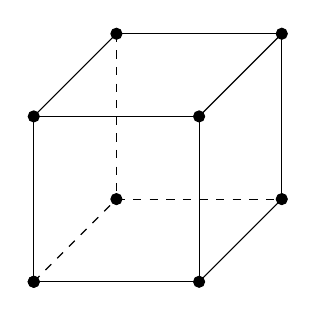
\begin{tikzpicture}[font = \large, scale = 0.7]
        \draw (3,0) -- (3,3);
        \draw (3,3) -- (0,3);
        \draw (0,3) -- (0,0);
        \draw (0,0) -- (3,0);
        
        \draw [dashed] (1.5,1.5) -- (4.5,1.5);
        \draw (4.5,1.5) -- (4.5,4.5);
        \draw (4.5,4.5) -- (1.5,4.5);
        \draw [dashed] (1.5,4.5) -- (1.5,1.5);
        
        \draw [dashed] (0,0) -- (1.5,1.5);
        \draw (3,0) -- (4.5,1.5);
        \draw (3,3) -- (4.5,4.5);
        \draw (0,3) -- (1.5,4.5);
        
        \draw [fill = black] (0,0) circle(1mm);
        \draw [fill = black] (3,0) circle(1mm);
        \draw [fill = black] (3,3) circle(1mm);
        \draw [fill = black] (0,3) circle(1mm);
        \draw [fill = black] (1.5,1.5) circle(1mm);
        \draw [fill = black] (4.5,1.5) circle(1mm);
        \draw [fill = black] (4.5,4.5) circle(1mm);
        \draw [fill = black] (1.5,4.5) circle(1mm);
        
        \draw [fill = black] (0,0) circle(1mm);
    \end{tikzpicture}
\end{figure}

\timestamp{1:06:05}
Данный граф не является плоским, однако он планарный и его можно перерисовать таким образом, чтобы он стал плоским.

\begin{figure}[H]
    \centering
    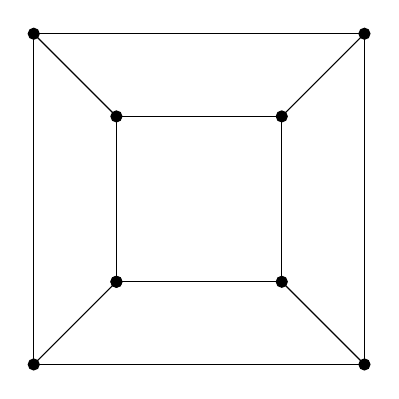
\begin{tikzpicture}[font = \large, scale = 0.7]
        \draw (0,0) -- (3,0) -- (3,3) -- (0,3) -- cycle;
        
        \draw (-1.5,-1.5) -- (-1.5,4.5) -- (4.5,4.5) -- (4.5,-1.5) -- cycle;
        
        \draw (0,0) -- (-1.5,-1.5);
        \draw (3,0) -- (4.5,-1.5);
        \draw (3,3) -- (4.5,4.5);
        \draw (0,3) -- (-1.5,4.5);
        
        \draw [fill = black] (0,0) circle(1mm);
        \draw [fill = black] (3,0) circle(1mm);
        \draw [fill = black] (3,3) circle(1mm);
        \draw [fill = black] (0,3) circle(1mm);
        \draw [fill = black] (-1.5,-1.5) circle(1mm);
        \draw [fill = black] (4.5,-1.5) circle(1mm);
        \draw [fill = black] (4.5,4.5) circle(1mm);
        \draw [fill = black] (-1.5,4.5) circle(1mm);
        
        \draw [fill = black] (0,0) circle(1mm);
    \end{tikzpicture}
\end{figure}
\end{example}

Число граней в данном графе будет таким же, как и в предыдущем графе. Каждой грани будет соответствовать один цикл, кроме внешней, потому что данную грань можно получить, складывая все остальные, поэтому можно сказать, что
\begin{equation}
    \text{Ц = Г} - 1
    \label{eq:1}
\end{equation}
\begin{note}
    Г - количество граней.
\end{note} 

\timestamp{1:08:05}
Кроме того, если мы рассматриваем связный граф или многогранник, то компонента связности будет только одна, т.е. $\text{К} = 1$.

Подставив полученное равенство в формулу Эйлера, получим формулу Эйлера для многогранников
$$ \text{В + Г} - 1 = \text{Р} + 1 \rightarrow \text{В + Г = Р} + 2$$
\begin{equation}
    \text{В + Г = Р} + 2
    \label{eq:tojdEylera}
\end{equation}

\newpage

\timestamp{1:09:30}
\section{Планарные графы}
Отметим, что существует всего два типа непланарных графов, все остальные можно к ним свести некоторыми специальными приемами.

\begin{figure}[H]
    \centering
    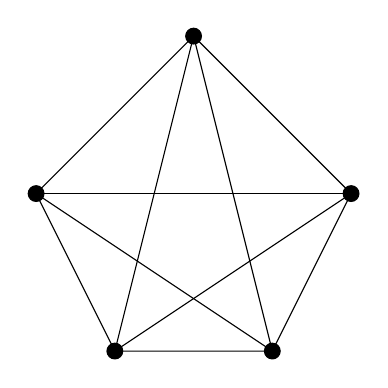
\begin{tikzpicture}[font = \large]
        \draw (0,0) -- (2,0) -- (3,2) -- (1,4) -- (-1,2) -- cycle;
        
        \draw (0,0) -- (3,2);
        \draw (0,0) -- (1,4);
        
        \draw (2,0) -- (1,4);
        \draw (2,0) -- (-1,2);
        
        \draw (-1,2) -- (3,2);
        
        \draw [fill = black] (0,0) circle(1mm);
        \draw [fill = black] (2,0) circle(1mm);
        \draw [fill = black] (3,2) circle(1mm);
        \draw [fill = black] (1,4) circle(1mm);
        \draw [fill = black] (-1,2) circle(1mm);
    \end{tikzpicture}
    \caption{Полный пятивершинный граф}
    \label{fig:3}
\end{figure}

\begin{note}
    Обозначается $K_5$. У данного графа 5 вершин, каждая из которых соединена со всеми остальными.
\end{note}

\begin{figure}[H]
    \centering
    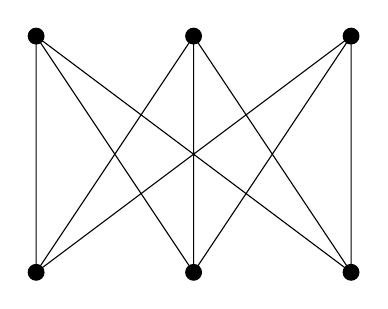
\begin{tikzpicture}[font = \large]
        \draw (0,0) -- (0,3) -- (2,0) -- (2,3) -- (4,0) -- (4,3) -- (0,0) -- (2,3) -- (2,0) -- (4,3) -- (4,0) -- (0,3);
        
        \draw [fill = black] (0,0) circle(1mm);
        \draw [fill = black] (0,3) circle(1mm);
        \draw [fill = black] (2,0) circle(1mm);
        \draw [fill = black] (2,3) circle(1mm);
        \draw [fill = black] (4,0) circle(1mm);
        \draw [fill = black] (4,3) circle(1mm);
    \end{tikzpicture}
    \caption{Двудольный полный граф 3 на 3}
    \label{fig:4}
\end{figure}
\begin{note}
    Обозначается $K_{3,3}$. Данный граф еще носит название "Три дома, три колодца".
\end{note}

С графом $K_{3,3}$ связана следующая головомка: необходимо от каждого дома   к каждому колодцу дорожки провести дорогу так, чтобы они не пересекались. Как бы вы не старались, все равно какие-нибудь две дорожки пересекутся.

\timestamp{1:11:30}
\begin{theorem}
    Графы $K_5$ и $K_{3,3}$ непланарны (нельзя нарисовать на плоскости без пересечений ребер, как бы мы не меняли расположение вершин).
\end{theorem}

\begin{proof}
    Пойдем от противного, пусть $K_5$ - планарный, тогда применим \hyperref[eq:tojdEylera]{тождество Эйлера} и найдем число граней:
$\text{Г = Р} + 2 - \text{В} = 7$

Можно ли данный граф перерисовать так, чтобы он стал плоским с числом граней равным 7?

\timestamp{1:13:45}
Рассмотрим грань с минимальным количеством ребер - это треугольник.

\begin{figure}[H]
    \centering
    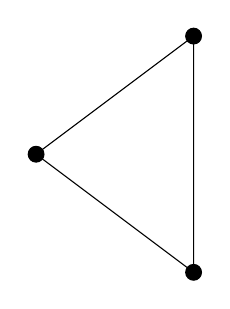
\begin{tikzpicture}[font = \large]
        \draw (0,1.5) -- (2,3) -- (2,0) -- cycle;
        
        \draw [fill = black] (0,1.5) circle(1mm);
        \draw [fill = black] (2,3) circle(1mm);
        \draw [fill = black] (2,0) circle(1mm);
    \end{tikzpicture}
\end{figure}

Тогда, даже если все грани содержат минимальное число рёбер, то их должно быть по крайней мере втрое больше, чем граней. Правда при этом каждое ребро мы посчитаем дважды (так как оно принадлежит двум соседним граням), из-за чего возникает необходимость поделить 3Г на 2. Отсюда, число рёбер в планарном графе не меньше $\frac{3\text{Г}}{2}$.

\begin{figure}[H]
    \centering
    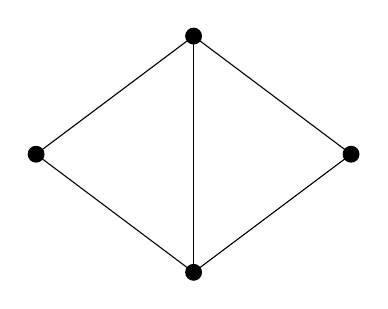
\begin{tikzpicture}[font = \large]
        \draw (0,1.5) -- (2,3) -- (4,1.5) -- (2,0) -- cycle;
        
        \draw (2,3) -- (2,0);
        
        \draw [fill = black] (0,1.5) circle(1mm);
        \draw [fill = black] (2,3) circle(1mm);
        \draw [fill = black] (2,0) circle(1mm);
        \draw [fill = black] (4,1.5) circle(1mm);
    \end{tikzpicture}
\end{figure}

\timestamp{1:14:50}
Тогда число рёбер в графе $K_5$ не меньше $\frac{3 \cdot 7}{2} = 10\frac{1}{2}$. Из-за чего возникает противоречие, т.к. число ребёр равно 10.

\timestamp{1:16:10}
Перейдем ко второму графу.

Попробуем применить те же соображения:  пусть $K_{3,3}$ - планарный, тогда число граней $\text{Г = Р +} \ 2 - \text{В = } 5$

Число рёбер в $K_{3,3}$ тогда не меньше $\frac{3 \cdot 5}{2} = 7 \frac{1}{2}$. Противоречия не возникает.

Вернемся к двудольному графу 3 на 3.

\timestamp{1:17:35}
\begin{note}
    Данный граф называется двудольным, потому что вершины можно раскрасить в два цвета так, что все рёбра будут соединять вершины разных цветов.
    
    \begin{figure}[H]
        \centering
        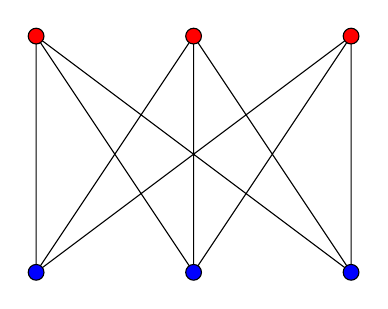
\begin{tikzpicture}[font = \large]
            \draw (0,0) -- (0,3) -- (2,0) -- (2,3) -- (4,0) -- (4,3) -- (0,0) -- (2,3) -- (2,0) -- (4,3) -- (4,0) -- (0,3);
            
            \draw [fill = blue] (0,0) circle(1mm);
            \draw [fill = red] (0,3) circle(1mm);
            \draw [fill = blue] (2,0) circle(1mm);
            \draw [fill = red] (2,3) circle(1mm);
            \draw [fill = blue] (4,0) circle(1mm);
            \draw [fill = red] (4,3) circle(1mm);
        \end{tikzpicture}
    \end{figure}

\end{note}

\timestamp{1:18:20}
Число рёбер в двудольном графе не может быть меньше 4Г, так как минимальное число ребер в грани четыре (если гранью является треугольник, то правильно раскрасить вершины в два цвета невозможно, в то время как исходный граф раскрашен в два цвета).

\begin{figure}[H]
    \centering
    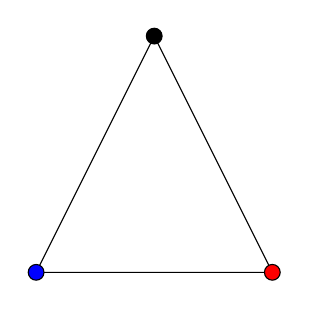
\begin{tikzpicture}[font = \large]
        \draw (0,0) -- (3,0) -- (1.5,3) -- cycle;
        
        \draw [fill = blue] (0,0) circle(1mm);
        \draw [fill = red] (3,0) circle(1mm);
        \draw [fill = black] (1.5,3) circle(1mm);
    \end{tikzpicture}
\end{figure}

\timestamp{1:18:50}
Поэтому для двудольного графа число рёбер в планарном графе не меньше  $\frac{4\text{Г}}{2} = 2\text{Г}$.

\begin{figure}[H]
    \centering
    \begin{tikzpicture}[font = \large]
        \draw (0,0) -- (3,0) -- (3,3) -- (0,3) -- cycle;
        
        \draw [fill = blue] (0,0) circle(1mm);
        \draw [fill = red] (3,0) circle(1mm);
        \draw [fill = blue] (3,3) circle(1mm);
        \draw [fill = red] (0,3) circle(1mm);
    \end{tikzpicture}
\end{figure}

Вернемся к нашему доказательству. $\text{Г = Р +} \ 2 - \text{В = } 5$, тогда число ребер при условии планарности должно быть по крайней мере в два раза больше Р = 2Г = 10. Но в графе К 3,3 их только 9, значит, и второй граф также не является планарным.

\end{proof}

\end{document} 
